% संपूर्ण मराठी ग्रंथातील प्रकरण 60: क्रमसूचक संख्या
% हा संपादनयोग्य स्रोतखंड आहे. संकलनासाठी संपूर्ण स्रोतसंग्रहातील
% अक्षररूपे, पूर्वभाग, चिन्हव्याख्या आणि आकृती-स्रोत आवश्यक आहेत.
% मूळ: Open Logic Project; मजकूर आणि रूपांतर CC BY 4.0.
% यंत्रानुवाद, दुरुस्ती आणि तपासणी: OpenAI Codex —
% GPT-5.6 Sol आणि GPT-6 Sol, दोन्ही Ultra effort.
% दुरुस्ती-पुनरावलोकन: GPT-6.1 Sol, Ultra effort.
\chapter{क्रमसूचक संख्या}\label{sth:ordinals:chap}









\section{प्रस्तावना}\label{sth:ordinals:intro:sec}

\ref{sth:z:chap} मध्ये \stagesinf{} या रूपात पदानुक्रमात अनंत टप्पा आहे असे आपण गृहीत धरले (अनंततेचे स्वयंसिद्धकही पाहा). पण \stagessucc{} मानल्यावर त्या टप्प्यावर थांबता येत नाही; पुढे जावेच लागते. म्हणून पहिल्या अनंत टप्प्यानंतरच्या टप्प्यावर त्या पहिल्या अनंत टप्प्यावर उपलब्ध असलेल्या संचांपासून बनणारे सर्व शक्य संग्रह तयार होतात; मग पुन्हा तेच; पुन्हा; पुन्हा; \dots

यात अप्रकटपणे आपण संख्येची एक ``सहज'' संकल्पना वापरू लागलो आहोत: सर्व नैसर्गिक संख्यांच्या \emph{नंतरही} संख्या असू शकतात. विशेषतः येथे अभिप्रेत आहे ती \emph{अनंतपार क्रमसूचक संख्या}. या कल्पनेला अधिक काटेकोर रूप देणे हे या प्रकरणाचे उद्दिष्ट आहे. आपण क्रमसूचक संख्यांची सर्वसाधारण संकल्पना पाहू आणि मग काही विशिष्ट संचांची स्पष्ट व्याख्या आपल्या क्रमसूचक संख्या म्हणून करू.







\section{क्रमसूचक संख्येची सर्वसाधारण कल्पना}\label{sth:ordinals:idea:sec}

नैसर्गिक संख्यांचा नेहमीचा क्रम पाहा:
\begin{center}
	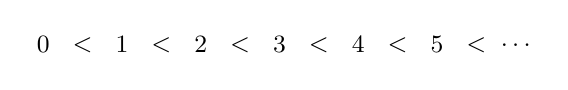
\begin{tikzpicture}
	\foreach \x/\xtext in {0, 1, 2, 3, 4, 5}
	{
		\node (\x a) at (\x, 1) {\small{$\x$}};
		\node (\x a) at (\x.5, 1) {\small{$<$}};
	}
	\node (ldots) at (6, 1) {\small{$\ldots$}};
	\end{tikzpicture}
\end{center}
याला तांत्रिक भाषेत $\omega$-अनुक्रम म्हणतात. संचांच्या पदानुक्रमातील सुरुवातीचे टप्पे बांधताना हीच सर्वसाधारण क्रमरचना दिसते. आता या अनुक्रमातील $0$ बाकी सर्व संख्यांच्या शेवटी नेऊ:
\begin{center}
	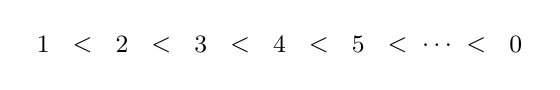
\begin{tikzpicture}
	\foreach \x/\xtext in {1, 2, 3, 4, 5}
	{
		\node (\x a) at (\x, 1) {\small{$\x$}};
		\node (\x a) at (\x.5, 1) {\small{$<$}};
	}
	\node (ldots) at (6, 1) {\small{$\ldots$}};
	\node (bea) at (6.5, 1) {\small{$<$}};
	\node (noa) at (7, 1) {\small{$0$}};
	\end{tikzpicture}
\end{center}
येथे घटक तेच आहेत; पण त्यांचा क्रम मुळात वेगळा आहे. पहिल्या क्रमाला शेवटचा घटक नव्हता; नव्या क्रमाला आहे. या नव्या क्रमात घटकांचा $\omega$-अनुक्रम ($1, 2, 3, 4, 5, \ldots$) आहे आणि त्यानंतर आणखी एक घटक येतो. म्हणून तो $\omega+1$-अनुक्रम आहे.

हेच घटक वापरून आणखी वेगवेगळ्या प्रकारचे क्रम बनवता येतात. उदाहरणार्थ, सर्व सम संख्या त्यांच्या नेहमीच्या क्रमात आणि त्यानंतर सर्व विषम संख्या त्यांच्या नेहमीच्या क्रमात घ्या:
\begin{center}
	\begin{tikzpicture}
	\node(a1) at (1,1) {\small{$0$}};
	\node(a2) at (1.5,1) {\small{$<$}};
	\node(a3) at (2,1) {\small{$2$}};
	\node(a4) at (2.5,1) {\small{$<$}};
	\node(a5) at (3,1) {\small{$4$}};
	\node(a6) at (3.5,1) {\small{$<$}};
	\node(dots) at (4,1) {\small{$\ldots$}};
	\node(aaoe) at (4.5,1) {\small{$<$}};
	\node(b1) at (5,1) {\small{$1$}};
	\node(b2) at (5.5,1) {\small{$<$}};
	\node(b3) at (6,1) {\small{$3$}};
	\node(b4) at (6.5,1) {\small{$<$}};
	\node(b5) at (7,1) {\small{$\ldots$}};
	\end{tikzpicture}
\end{center}
हा एका $\omega$-अनुक्रमानंतर दुसरा $\omega$-अनुक्रम आहे; म्हणजे $\omega+\omega$-अनुक्रम.

असे पुढेही करता येईल. पण \emph{क्रमरचनांविषयी} ही चर्चा समजून घेण्यासाठी आपल्याला एक सर्वसाधारण पद्धत हवी आहे.








\section{सुक्रमण}\label{sth:ordinals:wo:sec}

मूलभूत संकल्पना पुढीलप्रमाणे आहे:

\begin{defn}
$<\subseteq A\times A$ हा संबंध $A$ ला \emph{सुक्रमित करतो}
तेव्हा आणि केवळ तेव्हाच, जेव्हा पुढील दोन्ही अटी पूर्ण होतात:
\begin{enumerate}
\item $<$ हा जोडलेला असतो; म्हणजे सर्व $a, b \in A$ साठी $a < b$ किंवा $a = b$ किंवा $b < a$;
\item $A$ च्या प्रत्येक रिकाम्या नसलेल्या उपसंचात असा घटक असतो की त्या उपसंचातील कोणताही सदस्य त्याच्या $<$-आधी येत नाही; म्हणजे $\emptyset \neq X \subseteq A$ असल्यास $(\exists m \in
X)(\forall z \in X)z \nless m$.
\end{enumerate}
\end{defn}

आपण नुकत्याच पाहिलेल्या तिन्ही उदाहरणांतील क्रमसंबंध सुक्रमणच करतात, हे सहज दिसते.

\begin{prob}
\ref{sth:ordinals:idea:sec} मध्ये नैसर्गिक संख्यांवरील तीन क्रमांची उदाहरणे दिली. प्रत्येक क्रम सुक्रमण आहे, हे तपासा.
\end{prob}

सुक्रमणाबद्दल काही प्राथमिक पण अत्यंत महत्त्वाची निरीक्षणे पाहू.

\begin{prop}\label{sth:ordinals:wo:wo:strictorder}
$<$ हा $A$ ला सुक्रमित करत असेल, तर $A$ च्या प्रत्येक रिकाम्या नसलेल्या उपसंचात एकमेव $<$-लघुतम सदस्य असतो; शिवाय $<$ हा अपरावर्ती, असममित आणि संक्रमक असतो.
\end{prop}

\begin{proof}
$X$ हा $A$ चा रिकामा नसलेला उपसंच असेल, तर त्यात असा घटक $m$ असतो की $X$ मधील कोणताही सदस्य त्याच्या $<$-आधी येत नाही; म्हणजे $(\forall z \in X)z \nless m$. $<$ जोडलेला असल्याने $(\forall z \in X)m \leq z$. म्हणून $m$ हा $X$ मधील $<$-लघुतम घटक आहे.

अपरावर्तितेसाठी एखादा $a \in A$ निश्चित करू. $\{a\}$ चा $<$-लघुतम घटक $a$ असल्याने $a \nless a$. संक्रमकतेसाठी $a < b < c$ असेल, तर $\{a, b, c\}$ मध्ये $<$-लघुतम घटक असल्यामुळे $a < c$. अपरावर्तिता आणि संक्रमकता यांवरून असममिती मिळते.
\end{proof}

\begin{prop}\label{sth:ordinals:wo:propwoinduction}
$<$ हा $A$ ला सुक्रमित करत असेल, तर कोणत्याही सूत्र $\phi(x)$ साठी:
\[
\text{जर }(\forall a \in A)((\forall b < a)\phi(b) \lif
\phi(a))\text{, तर }(\forall a \in A)\phi(a).
\]
\end{prop}

\begin{proof}
व्यत्यस्त रूप सिद्ध करू. $\lnot(\forall a \in
A)\phi(a)$, म्हणजे $X = \Setabs{x \in A}{\lnot\phi(x)} \neq
\emptyset$, असे मानू. मग $X$ मध्ये पूर्ववर्ती नसलेला घटक $a$ असतो. म्हणून $(\forall
b < a)\phi(b)$; पण $\lnot \phi(a)$.
\end{proof}\noindent हा शेवटचा गुणधर्म नैसर्गिक संख्यांवरील प्रबल विगमनाच्या तत्त्वाची आठवण करून देतो: $(\forall n \in \omega)((\forall m < n)\phi(m)
\lif \phi(n))$ असेल, तर $(\forall n \in \omega)\phi(n)$. त्यामुळे सुक्रमण ही फार \emph{भक्कम} संकल्पना ठरते.\footnote{आठवण: स्पष्टपणे अन्यथा सांगितले नसेल, तर सर्व सूत्रांत प्राचले असू शकतात.}








\section{क्रम-समरूपणे}\label{sth:ordinals:iso:sec}

सुक्रमण किती \emph{भक्कम} आहे, हे स्पष्ट करण्यासाठी आपण सुक्रमणांची तुलना करण्याची एक पद्धत आधी मांडू.

\begin{defn}
$<$ हा $A$ ला सुक्रमित करत असेल, तर $\tuple{A, <}$ या जोडीला \emph{सुक्रमण} म्हणतात. $\tuple{A, <}$ आणि $\tuple{B,
\lessdot}$ ही सुक्रमणे \emph{क्रम-समरूपी} असतात तेव्हा आणि केवळ तेव्हाच, जेव्हा $f \colon A \to B$ असे एकास-एक आच्छादन असते की: $x < y$ तेव्हा आणि केवळ तेव्हाच $f(x) \lessdot  f(y)$. अशा वेळी $\ordeq{\tuple{A, <}}{\tuple{B, \lessdot}}$ असे लिहितो आणि $f$ ला \emph{क्रम-समरूपण} म्हणतो.
\end{defn}
\noindent
पुढे संक्षेपासाठी आपण ``क्रम-समरूपणे'' यांऐवजी ``समरूपणे'' असे म्हणू. सहज अर्थाने, समरूपणे म्हणजे रचना जपणारी एकास-एक आच्छादने असतात. त्यांच्याबद्दल काही साधी तथ्ये पुढे दिली आहेत.

\begin{lem}\label{sth:ordinals:iso:isoscompose}
समरूपणांची संयुक्तीही समरूपण असते. म्हणजे, $f \colon A
\to B$ आणि $g \colon B \to C$ ही समरूपणे असतील, तर $(g \circ f)
\colon A \to C$ हेही समरूपण असते.
\end{lem}
\begin{prob}
	\ref{sth:ordinals:iso:isoscompose} सिद्ध करा.
\end{prob}
\begin{proof}
हा पुरावा सरावासाठी सोडला आहे.
\end{proof}
\begin{cor}\label{sth:ordinals:iso:ordisoisequiv}
	$\ordeq{X}{Y}$ हा समतुल्यता संबंध आहे.
\end{cor}
\begin{prop}\label{sth:ordinals:iso:ordisounique}
$\tuple{A, <}$ आणि $\tuple{B, \lessdot}$ ही समरूपी सुक्रमणे असतील, तर त्यांच्यामधील समरूपण एकमेव असते.
\end{prop}

\begin{proof}
$f$ आणि $g$ ही $A \to B$ समरूपणे मानू. \ref{sth:ordinals:wo:propwoinduction} वापरून विगमनाने हा निष्कर्ष सिद्ध करू.
$a\in A$ निश्चित करू आणि विगमनाच्या गृहीतकानुसार $(\forall b < a)f(b) = g(b)$ मानू. $x \in B$ निश्चित करू.

$x \lessdot f(a)$ असेल, तर $f^{-1}(x) < a$. $f$ आणि $g$ ही समरूपणे असल्यामुळे $g(f^{-1}(x)) \lessdot
g(a)$. पण $f^{-1}(x) < a$ असल्याने आपल्या गृहीतकावरून $x =f(f^{-1}(x)) = g(f^{-1}(x))$ मिळते. म्हणून $x \lessdot g(a)$. त्याचप्रमाणे, $x \lessdot g(a)$ असल्यास $x \lessdot
f(a)$.

म्हणून $(\forall x \in B)(x \lessdot f(a) \liff x \lessdot
g(a))$. \ref{sfr:rel:ord:prop:extensionality-strictlinearorders} वरून $f(a) = g(a)$ मिळते. त्यामुळे \ref{sth:ordinals:wo:propwoinduction} वरून $(\forall
a \in A)f(a) = g(a)$.
\end{proof}\noindent
यावरून सुक्रमणाचे भक्कम स्वरूप काहीसे स्पष्ट होते. ते अधिक समजण्यासाठी आणखी काही संज्ञा निश्चित करू.

\begin{defn}
$\tuple{A, <}$ हे सुक्रमण आणि $a \in A$ असेल, तर $A_a = \Setabs{x \in A}{x
< a}$ असे मानू. $A_a$ हा $A$ चा यथार्थ \emph{आरंभीचा खंड} आहे असे म्हणू; $A$ स्वतःही $A$ चा अयथार्थ आरंभीचा खंड असू शकतो. $<_a$ हा आरंभीच्या खंडापुरता $<$ चा संकोच, म्हणजे $\funrestrictionto{\mathord{<}}{A_a^2}$, मानू.
\end{defn}
\noindent
या संज्ञांद्वारे कोणतेही सुक्रमण स्वतःच्या यथार्थ आरंभीच्या खंडाशी समरूपी नसते, हे मांडता आणि सिद्ध करता येते.

\begin{lem}\label{sth:ordinals:iso:wellordnotinitial}
$\tuple{A, <}$ हे सुक्रमण आणि $a \in A$ असेल, तर
$\ordneq{\tuple{A, <}}{\tuple{A_a, <_a}}$.
\end{lem}

\begin{proof}
विसंगतीसाठी $f \colon A \to A_a$ हे समरूपण आहे असे मानू. $f$ हे एकास-एक आच्छादन असून $A_a \subsetneq A$ असल्याने, \ref{sth:ordinals:wo:wo:strictorder} वापरून $A$ मधील $b \neq f(b)$ पूर्ण करणारा $<$-लघुतम घटक $b \in A$ घेऊ. $(\forall x \in A)(x<b \liff x < f(b))$ हे दाखवू. मग \ref{sfr:rel:ord:prop:extensionality-strictlinearorders} वरून $b = f(b)$ मिळेल आणि विसंगती सिद्ध होईल.

$x < b$ मानू. $b$ च्या निवडीवरून $x = f(x)$. तसेच $f$ समरूपण असल्याने $f(x) < f(b)$. म्हणून $x < f(b)$.

$x < f(b)$ मानू. $f$ समरूपण असल्याने $f^{-1}(x) < b$; म्हणून $b$ च्या निवडीवरून $f^{-1}(x) = x$. त्यामुळे $x < b$.
\end{proof}

पुढील निष्कर्ष साधारणपणे असे सांगतो की समरूपणाचा ``आरंभीचा खंड'' हाही समरूपण असतो:

\begin{lem}\label{sth:ordinals:iso:wellordinitialsegment}
$\tuple{A, <}$ आणि $\tuple{B, \lessdot}$ ही सुक्रमणे मानू. $f
\colon A \to B$ हे समरूपण आणि $a \in A$ असेल, तर
$\funrestrictionto{f}{A_{a}} : A_a \to B_{f(a)}$ हे समरूपण असते.
\end{lem}

\begin{proof}
$f$ हे समरूपण असल्यामुळे:

\begin{align*}
	\funimage{f}{A_a} &= \funimage{f}{\Setabs{x \in A}{x < a}}\\
	&= \funimage{f}{\Setabs{f^{-1}(y) \in A}{f^{-1}(y) < a}} \\
	&= \Setabs{y \in B}{y \lessdot f(a)} \\
	&=B_{f(a)}
\end{align*}
मिळते. $f$ क्रम जपत असल्यामुळे $\funrestrictionto{f}{A_a}$ सुद्धा क्रम जपते.
\end{proof}

पुढील दोन निष्कर्षांवरून कोणतीही दोन सुक्रमणे तुलना करता येतात, हे सिद्ध होते:

\begin{lem}\label{sth:ordinals:iso:lemordsegments}
$\tuple{A, <}$ आणि $\tuple{B, \lessdot}$ ही सुक्रमणे मानू. जर
$\ordeq{\tuple{A_{a_1}, <_{a_1}}}{\tuple{B_{b_1}, \lessdot_{b_1}}}$
आणि $\ordeq{\tuple{A_{{a_2}}, <_{a_2}}}{\tuple{B_{{b_2}},
\lessdot_{b_2}}}$ असेल, तर ${a_1}  < {a_2} \text{ तेव्हा आणि केवळ तेव्हाच }{b_1} \lessdot
{b_2}$.
\end{lem}

\begin{proof}
\emph{डावीकडून उजवीकडे} हे सिद्ध करू; उलट दिशा तशीच आहे.
$\ordeq{\tuple{A_{a_1}, <_{a_1}}}{\tuple{B_{b_1},
\lessdot_{b_1}}}$ आणि $\ordeq{\tuple{A_{{a_2}},
<_{a_2}}}{\tuple{B_{{b_2}}, \lessdot_{b_2}}}$ दोन्ही मानू आणि $f \colon
A_{{a_2}} \to B_{{b_2}}$ हे समरूपण असू द्या. ${a_1} < {a_2}$ असेल, तर
\ref{sth:ordinals:iso:wellordinitialsegment} वरून
$\ordeq{\tuple{A_{a_1}, <_{a_1}}}{\tuple{B_{f({a_1})},
\lessdot_{f({a_1})}}}$ मिळते. म्हणून
$\ordeq{\tuple{B_{b_1}, \lessdot_{b_1}}}{\tuple{B_{f({a_1})},
\lessdot_{f({a_1})}}}$; आणि \ref{sth:ordinals:iso:wellordnotinitial} वरून ${b_1} = f({a_1})$. आता $f$ चे सहप्रांत $B_{{b_2}}$ असल्याने ${b_1} \lessdot {b_2}$.
\end{proof}

\begin{thm}\label{sth:ordinals:iso:thm:woalwayscomparable}
कोणतीही दोन सुक्रमणे दिल्यास, त्यांपैकी एक दुसऱ्याच्या आरंभीच्या खंडाशी समरूपी असते; तो खंड यथार्थ असलाच पाहिजे असे नाही.
\end{thm}

\begin{proof}
$\tuple{A, <}$ आणि $\tuple{B, \lessdot}$ ही सुक्रमणे मानू. विभक्तीकरण वापरून
\[
	f = \Setabs{\tuple{a, b} \in A \times B}{
		\ordeq{\tuple{A_a, <_a}}{\tuple{B_b, \lessdot_b}}}.
\]
असे ठरवू. \ref{sth:ordinals:iso:lemordsegments} वरून $\tuple{a_1, b_1}, \tuple{a_2, b_2} \in f$ अशा सर्व जोड्यांसाठी $a_1 < a_2$ तेव्हा आणि केवळ तेव्हाच $b_1 \lessdot b_2$. म्हणून $f \colon \dom{f} \to
\ran{f}$ हे समरूपण आहे.

$a_2 \in \dom{f}$ आणि $a_1 < a_2$ असेल, तर \ref{sth:ordinals:iso:wellordinitialsegment} वरून $a_1 \in \dom{f}$; म्हणून $\dom{f}$ हा $A$ चा आरंभीचा खंड आहे. त्याचप्रमाणे $\ran{f}$ हा $B$ चा आरंभीचा खंड आहे. विसंगतीसाठी हे दोन्ही \emph{यथार्थ} आरंभीचे खंड आहेत असे मानू. मग $A \setminus \dom{f}$ मधील $<$-लघुतम घटक $a$ घेऊ; त्यामुळे $\dom{f} = A_a$. तसेच $B \setminus
\ran{f}$ मधील $\lessdot$-लघुतम घटक $b$ घेऊ; त्यामुळे $\ran{f} = B_b$. म्हणून $f \colon A_a \to B_b$ हे समरूपण आहे आणि त्यामुळे $\tuple{a, b} \in f$; ही विसंगती आहे.
\end{proof}







\section{क्रमसूचक संख्यांची फोन न्यूमनची रचना}\label{sth:ordinals:vn:sec}

\ref{sth:ordinals:iso:thm:woalwayscomparable} वरून एक कल्पना सुचते. सुक्रमणांचे प्रतिनिधी म्हणून \emph{क्रमप्रकार} नावाच्या काही वस्तू आपण मांडू शकतो. $\tuple{A, <}$ या सुक्रमणाचा क्रमप्रकार $\ordtype{A, <}$ असा लिहू; मग पुढील दोन तत्त्वे मिळतील अशी अपेक्षा असेल:
\begin{align*}
	\ordtype{A, <} = \ordtype{B, \lessdot} &
	\text{ तेव्हा आणि केवळ तेव्हाच } \ordeq{\tuple{A, <}}{\tuple{B, \lessdot}}\\
	\ordtype{A, <} < \ordtype{B, \lessdot}&
	\text{ तेव्हा आणि केवळ तेव्हाच }\ordeq{\tuple{A, <}}{\tuple{B_b, \lessdot_b}}\text{ असे काही }b \in B
\end{align*}
शिवाय, नैसर्गिक संख्या जशा विशिष्ट संचांच्या रूपात मांडता येतात, तसे क्रमप्रकारही \emph{विशिष्ट संचांच्या रूपात} मांडता येतील अशी अपेक्षा असू शकते.

ते करण्याची सर्वाधिक प्रचलित पद्धत---आणि आपण अनुसरणार असलेली पद्धत---म्हणजे विशिष्ट \emph{प्रमाणभूत} सुक्रमित संचांच्या आधारे हे क्रमप्रकार परिभाषित करणे. असे प्रमाणभूत संच प्रथम फोन न्यूमन यांनी मांडले:

\begin{defn}
$(\forall x \in A)x \subseteq A$ असेल तेव्हा आणि केवळ तेव्हाच $A$ हा संच \emph{संक्रमक} असतो. $A$ हा संक्रमक असून त्याच्या सदस्यांपुरत्या $\in$ च्या बंधनाने सुक्रमित असेल तेव्हा आणि केवळ तेव्हाच $A$ ही \emph{क्रमसूचक संख्या} असते.
\end{defn}
\noindent
यापुढे क्रमसूचक संख्यांसाठी ग्रीक अक्षरे वापरू. व्याख्येवरून लगेच दिसते की $\alpha$ ही क्रमसूचक संख्या असल्यास $\tuple{\alpha, \in_\alpha}$ हे सुक्रमण आहे; येथे $\in_\alpha =
\Setabs{\tuple{x, y} \in \alpha^2}{x \in y}$. म्हणून संकेतलेखनात किंचित मोकळीक घेऊन $\alpha$ \emph{स्वतःच} एक सुक्रमण आहे असेही म्हणू शकतो.

पहिल्या काही क्रमसूचक संख्या पुढीलप्रमाणे आहेत:
\[
	\emptyset, \{\emptyset\},
	\{\emptyset, \{\emptyset\}\},
	\{\emptyset, \{\emptyset\}, \{\emptyset, \{\emptyset\}\}\}, \ldots
\]
अनंततेच्या स्वयंसिद्धकात, म्हणजे फोन न्यूमन यांच्या $\omega$ च्या व्याख्येत, आपल्याला भेटलेल्या पहिल्या काही क्रमसूचक संख्या याच आहेत (\ref{sth:z:infinity-again:sec} पाहा). हा योगायोग नाही. फोन न्यूमन यांच्या व्याख्येत नैसर्गिक संख्या क्रमसूचक संख्या असतात; पण अनंतपार क्रमसूचक संख्यांनाही जागा असते.

नेहमीप्रमाणे आता विचारता येईल: \emph{याच} क्रमसूचक संख्या आहेत का? की फोन न्यूमन यांनी आपल्याला असे काही संच दिले आहेत ज्यांना आपण क्रमसूचक संख्या \emph{मानू शकतो}? या प्रश्नावरील चर्चा \ref{sfr:rel:ref:sec}, \ref{sfr:arith:ref:sec}, \ref{sfr:infinite:dedekindsproof:sec} आणि \ref{sth:z:nat:sec} मधील चर्चांप्रमाणेच आहे; म्हणून येथे ती पुन्हा विस्ताराने करणार नाही. पुढे ``क्रमसूचक संख्या'' म्हटल्यावर आपण ``फोन न्यूमन यांच्या क्रमसूचक संख्या'' अभिप्रेत धरू.







\section{क्रमसूचक संख्यांचे मूलभूत गुणधर्म}\label{sth:ordinals:basic:sec}

पहिल्या काही क्रमसूचक संख्या नैसर्गिक संख्याच आहेत, हे आपण पाहिले. क्रमसूचक संख्यांची उपपत्ती विकसित करण्यामागचा मुख्य उद्देश म्हणजे नैसर्गिक संख्यांसाठी लागू असलेले विगमनाचे तत्त्व पुढे नेणे. काही प्राथमिक निष्कर्षांच्या साहाय्याने आपण ते साध्य करू.

\begin{lem}\label{sth:ordinals:basic:ordmemberord}
क्रमसूचक संख्येचा प्रत्येक घटक ही क्रमसूचक संख्या असतो.
\end{lem}

\begin{proof}
$\alpha$ ही क्रमसूचक संख्या आणि $b \in \alpha$ असे मानू. $\alpha$ संक्रमक असल्याने $b \subseteq \alpha$. त्यामुळे $\in$ जसा $\alpha$ ला सुक्रमित करतो, तसाच $\in$ हा $b$ लाही सुक्रमित करतो.

$b$ संक्रमक आहे हे पाहण्यासाठी $x \in c \in b$ मानू. $b
\subseteq \alpha$ असल्याने $c \in \alpha$. पुन्हा $\alpha$ संक्रमक असल्याने $c \subseteq
\alpha$ आणि म्हणून $x \in \alpha$. अशा प्रकारे $x, c, b \in \alpha$. पण $\in$ हा $\alpha$ ला सुक्रमित करतो; म्हणून \ref{sth:ordinals:wo:wo:strictorder} वरून $\in$ हा $\alpha$ वरील संक्रमक संबंध आहे. त्यामुळे $x
\in c \in b$ वरून $x \in b$. याचे सामान्यीकरण केल्यास $c \subseteq b$.
\end{proof}

\begin{cor}\label{sth:ordinals:basic:ordissetofsmallerord}
कोणत्याही क्रमसूचक संख्या~$\alpha$ साठी $\alpha = \Setabs{\beta \in \alpha}{\beta \text{ ही क्रमसूचक संख्या आहे}}$.
\end{cor}

\begin{proof}
\ref{sth:ordinals:basic:ordmemberord} वरून थेट मिळते.
\end{proof}

पुढील दोन मुख्य निष्कर्षांचा, \ref{sth:ordinals:basic:ordinductionschema} आणि \ref{sth:ordinals:basic:ordtrichotomy} यांचा, साधारण आशय असा की क्रमसूचक संख्याच सदस्यत्वाने सुक्रमित होतात:

\begin{thm}[अनंतपार विगमन]\label{sth:ordinals:basic:ordinductionschema}
कोणत्याही सूत्र $\phi(x)$ साठी:
\[
	\text{जर }\exists \alpha \phi(\alpha)\text{, तर }\exists \alpha(\phi(\alpha)
	\land  (\forall \beta \in \alpha) \lnot \phi(\beta))
\]
येथे दाखवलेली परिमाणके अव्यक्तपणे क्रमसूचक संख्यांपुरती मर्यादित आहेत.
\end{thm}

\begin{proof}

एखाद्या क्रमसूचक संख्या $\alpha$ साठी $\phi(\alpha)$ मानू. $ (\forall \beta
\in \alpha) \lnot \phi(\beta)$ असेल, तर सिद्धता झाली. अन्यथा, $\alpha$ ही क्रमसूचक संख्या असल्याने तिच्यात $\phi$ पूर्ण करणारा $\in$-लघुतम घटक मिळतो; \ref{sth:ordinals:basic:ordmemberord} वरून तोही क्रमसूचक संख्या आहे.






\end{proof}
\noindent
\ref{sth:ordinals:basic:ordinductionschema} हेच तत्त्व पुढील रूपबंधातही मांडता येते:
\[
\text{जर }\forall \alpha((\forall \beta \in \alpha)\phi(\beta) \lif
\phi(\alpha))\text{, तर }\forall \alpha\phi(\alpha)
\]
यासाठी \ref{sth:ordinals:basic:ordinductionschema} मध्ये $\lnot\phi(\alpha)$ घेऊन प्राथमिक तार्किक रूपांतरे करावी लागतात.

\begin{thm}[त्रिपर्याय]\label{sth:ordinals:basic:ordtrichotomy}
कोणत्याही क्रमसूचक संख्या $\alpha$ आणि $\beta$ साठी $\alpha \in \beta \lor \alpha = \beta \lor \beta \in \alpha$.
\end{thm}

\begin{proof}
पुरावा द्विगुण विगमनाने, म्हणजे \ref{sth:ordinals:basic:ordinductionschema} दोनदा वापरून, करता येतो. $x \in y \lor x = y \lor y \in x$ असेल तेव्हा आणि केवळ तेव्हाच $x$ आणि $y$ \emph{तुलनीय} आहेत असे म्हणू.

विगमनासाठी, $\alpha$ मधील प्रत्येक क्रमसूचक संख्या \emph{प्रत्येक} क्रमसूचक संख्येशी तुलनीय आहे असे मानू. आणखी एका विगमनासाठी, $\alpha$ ही $\beta$ मधील प्रत्येक क्रमसूचक संख्येशी तुलनीय आहे असे मानू. आता $\alpha$ ही $\beta$ शी तुलनीय आहे हे दाखवू. मग $\beta$ वरील विगमनाने $\alpha$ प्रत्येक क्रमसूचक संख्येशी तुलनीय ठरेल; आणि $\alpha$ वरील विगमनाने \emph{प्रत्येक} क्रमसूचक संख्या \emph{प्रत्येक} क्रमसूचक संख्येशी तुलनीय ठरेल, हेच हवे आहे. $\alpha \notin \beta$ आणि $\beta \notin
\alpha$ असे मानून $\alpha = \beta$ दाखवणे पुरेसे आहे.

$\alpha \subseteq \beta$ दाखवण्यासाठी $\gamma \in \alpha$ निश्चित करू; \ref{sth:ordinals:basic:ordmemberord} वरून ती क्रमसूचक संख्या आहे. म्हणून पहिल्या विगमन गृहीतकानुसार $\gamma$ ही $\beta$ शी तुलनीय आहे. पण $\gamma
= \beta$ किंवा $\beta \in \gamma$ यांपैकी काहीही असेल, तर $\beta \in \alpha$ मिळते (गरज पडल्यास $\alpha$ च्या संक्रमकतेचा वापर करून); हे आपल्या गृहीतकाविरुद्ध आहे. म्हणून $\gamma \in \beta$. याचे सामान्यीकरण केल्यास $\alpha \subseteq
\beta$.

दुसरे विगमन गृहीतक वापरून अगदी त्याच प्रकारच्या तर्काने $\beta \subseteq \alpha$ मिळते. म्हणून $\alpha = \beta$.
\end{proof}\noindent त्यामुळे कधी कधी $\alpha \in \beta$ ऐवजी $\alpha <\beta$ असे लिहू; कारण $\in$ येथे क्रमसंबंधाप्रमाणे वागतो. यामागे परिचय आणि $\alpha \in
\beta \lor \alpha = \beta$ याऐवजी $\alpha \leq \beta$ लिहिण्याची सोय यांपलीकडे विशेष कारण नाही.\footnote{$\alpha
\mathrel{\underline{\in}} \beta$ असेही लिहिता येईल; पण हा संकेत सर्वमान्य नाही.}

आपल्या मागील निष्कर्षांवरून पुढील दोन परिणाम लगेच मिळतात; पहिल्यात आपला नवा संकेत वापरला आहे:

\begin{cor}\label{sth:ordinals:basic:ordordered}
$\exists \alpha\phi(\alpha)$ असेल, तर $\exists \alpha(\phi(\alpha)
\land \forall \beta(\phi(\beta) \lif \alpha \leq \beta))$.
शिवाय, कोणत्याही क्रमसूचक संख्या $\alpha, \beta, \gamma$ साठी $\alpha
\notin \alpha$ आणि $\alpha \in \beta \in \gamma \lif \alpha \in
\gamma$.
\end{cor}

\begin{proof}
\ref{sth:ordinals:wo:wo:strictorder} प्रमाणेच.
\end{proof}

\begin{prob}
\ref{sth:ordinals:basic:ordtrichotomy} च्या पुराव्यातील ``अगदी त्याच प्रकारचा तर्क'' पूर्ण लिहा.
\end{prob}

\begin{cor}\label{sth:ordinals:basic:corordtransitiveord}
$A$ ही क्रमसूचक संख्या असते तेव्हा आणि केवळ तेव्हाच $A$ हा क्रमसूचक संख्यांचा संक्रमक संच असतो.
\end{cor}

\begin{proof}
\emph{डावीकडून उजवीकडे.} \ref{sth:ordinals:basic:ordmemberord} वरून. \emph{उजवीकडून डावीकडे.} $A$ हा क्रमसूचक संख्यांचा संक्रमक संच असेल, तर \ref{sth:ordinals:basic:ordinductionschema} आणि \ref{sth:ordinals:basic:ordtrichotomy} वरून $\in$ हा $A$ ला सुक्रमित करतो.
\end{proof}

\ref{sth:ordinals:basic:ordinductionschema} आणि \ref{sth:ordinals:basic:ordtrichotomy} यांचा आशय आपण क्रमसूचक संख्या $\in$ ने सुक्रमित होतात असा सांगितला. पण पुढील निष्कर्षामुळे असे विधान करताना \emph{फार सावध} राहिले पाहिजे:

\begin{thm}[बुराली-फोर्ती विरोधापत्ती]\label{sth:ordinals:basic:buraliforti}
सर्व क्रमसूचक संख्यांचा संच अस्तित्वात नाही.
\end{thm}

\begin{proof}
विसंगतीसाठी $O$ हा सर्व क्रमसूचक संख्यांचा संच आहे असे मानू. $\alpha \in
\beta \in O$ असेल, तर \ref{sth:ordinals:basic:ordmemberord} वरून $\alpha$ ही क्रमसूचक संख्या आहे आणि म्हणून $\alpha \in O$. त्यामुळे $O$ संक्रमक आहे; म्हणून \ref{sth:ordinals:basic:corordtransitiveord} वरून $O$ ही क्रमसूचक संख्या ठरते. मग $O \in O$, हे \ref{sth:ordinals:basic:ordordered} ला विरोधी आहे.
\end{proof}
\noindent
हा निष्कर्ष बुराली-फोर्ती यांच्या नावाने ओळखला जातो. परंतु सर्व क्रमसूचक संख्यांचा संच आहे असे मानल्यास \emph{विसंगती} निर्माण होते, हे १८९९ मध्ये डेडेकिंड यांना लिहिलेल्या पत्रात प्रथम स्पष्टपणे कांटोर यांच्या लक्षात आले. व्हान हायेनूर्ट यांनी सांगितल्याप्रमाणे:
\begin{quote}
  बुराली-फोर्ती यांनी स्वतः या विसंगतीतून \emph{विसंगतीद्वारे सिद्धतेने} असा निष्कर्ष काढला की क्रमसूचक संख्यांचा नैसर्गिक क्रम हा केवळ आंशिक क्रम आहे.
  (व्हान हायेनूर्ट 1967, पृ.~105)
\end{quote}
बुराली-फोर्ती यांची चूक बाजूला ठेवून आतापर्यंतचे निष्कर्ष असे सांगता येतील: क्रमसूचक संख्या या प्रत्येकी सदस्यत्वाने सुक्रमित संच असतात आणि एकत्रितपणेही सदस्यत्वाने सुक्रमित असतात; मात्र त्या एकत्रितपणे संच बनवत नाहीत.

हा भाग पूर्ण करण्यासाठी \ref{sth:ordinals:basic:ordinductionschema} आणि \ref{sth:ordinals:basic:ordtrichotomy} वरून मिळणारे क्रमसूचक संख्यांचे आणखी काही मूलभूत गुणधर्म पाहू.

\begin{prop}
क्रमसूचक संख्यांचा कोणताही काटेकोरपणे उतरणारा अनुक्रम परिमित असतो.
\end{prop}

\begin{proof}
क्रमसूचक संख्यांचा अनंत काटेकोरपणे उतरणारा अनुक्रम $\alpha_0 > \alpha_1 > \alpha_2 > \ldots$ असता, तर त्याच्या सदस्यांत $<$-लघुतम सदस्य नसता; हे \ref{sth:ordinals:basic:ordinductionschema} शी विसंगत आहे.
\end{proof}

\begin{prop}\label{sth:ordinals:basic:ordinalsaresubsets}
कोणत्याही क्रमसूचक संख्या $\alpha, \beta$ साठी $\alpha \subseteq \beta \lor \beta \subseteq \alpha$.
\end{prop}

\begin{proof}
$\alpha \in \beta$ असेल, तर $\beta$ संक्रमक असल्यामुळे $\alpha \subseteq \beta$. त्याचप्रमाणे $\beta \in \alpha$ असेल, तर $\beta \subseteq
\alpha$. आणि $\alpha = \beta$ असेल, तर $\alpha \subseteq \beta$ आणि $\beta \subseteq \alpha$. म्हणून \ref{sth:ordinals:basic:ordtrichotomy} वरून निष्कर्ष मिळतो.
\end{proof}

\begin{prop}\label{sth:ordinals:basic:ordisoidentity}
कोणत्याही क्रमसूचक संख्या $\alpha, \beta$ साठी $\alpha = \beta$ तेव्हा आणि केवळ तेव्हाच $\ordeq{\alpha}{\beta}$.
\end{prop}

\begin{proof}
क्रमसूचक संख्या या सुक्रमणे आहेत; म्हणून त्रिपर्याय (\ref{sth:ordinals:basic:ordtrichotomy}) आणि \ref{sth:ordinals:iso:wellordnotinitial} वरून हे लगेच मिळते.
\end{proof}

\begin{prob}\label{sth:ordinals:basic:probunionordinalsordinal}
$X$ चा प्रत्येक सदस्य क्रमसूचक संख्या असेल, तर $\bigcup X$ ही क्रमसूचक संख्या असते, हे सिद्ध करा.
\end{prob}








\section{प्रतिस्थापन}\label{sth:ordinals:replacement:sec}

\ref{sth:ordinals:vn:sec} मध्ये क्रमसूचक संख्यांना क्रमप्रकार म्हणून, म्हणजे सुक्रमणांचे प्रमाणभूत प्रतिनिधी म्हणून, घेता येईल असे सुचवून त्यांची ओळख करून दिली. हे साधण्यासाठी \emph{प्रत्येक सुक्रमण कोणत्या तरी क्रमसूचक संख्येशी समरूपी आहे} हे सिद्ध करावे लागेल. मग $\tuple{A, <} \isomorphic \alpha$ अशी क्रमसूचक संख्या $\alpha$ घेऊन $\ordtype{A, <}$ परिभाषित करता येईल.

दुर्दैवाने, आतापर्यंत आपण दिलेल्या स्वयंसिद्धकांवरून हा अपेक्षित निष्कर्ष \emph{सिद्ध करता येत नाही}. का ते \ref{sth:replacement:strength:sec} मध्ये पाहू; सध्या इतके लक्षात ठेवू की तो सिद्ध होत नाही. म्हणून आपल्याला एक नवे तत्त्व हवे आहे:

\begin{axiom}[प्रतिस्थापन-रूपबंध]
कोणत्याही सूत्र $\phi(x, y)$ साठी पुढील विधान हे एक स्वयंसिद्धक आहे:
\begin{quote}
	कोणत्याही $A$ साठी, $(\forall x \in A)\lexists![y][\phi(x,y)]$ असेल, तर $\Setabs{y}{(\exists x \in A)\phi(x,y)}$ अस्तित्वात असतो.
\end{quote}
\end{axiom}
\noindent
विभक्तीकरणाप्रमाणे हाही एक रूपबंध आहे: अनंत संख्येने असलेल्या निरनिराळ्या $\phi$ साठी त्यातून अनंत संख्येने स्वयंसिद्धके मिळतात. हेच तत्त्व पुढीलप्रमाणेही लिहिता येते, आणि सामान्यतः तसेच लिहिले जाते:

\begin{defish}
``$B$'' नसलेल्या कोणत्याही सूत्र $\phi(x,y)$ साठी पुढील विधान हे एक स्वयंसिद्धक आहे:
\[
\forall A[(\forall x \in A)\lexists![y][\phi(x,y)] \lif \exists B\forall y (y \in B \liff (\exists x \in A)\phi(x,y))]
\]
\end{defish}

पहिल्यांदा पाहताना हे सूत्र गुंतागुंतीचे वाटते. प्रतिस्थापनाचा पुढील सोपा परिणाम मात्र त्यामागील कल्पना \emph{अधिक स्पष्टपणे} व्यक्त करतो:\footnote{पद म्हणजे अशी अभिव्यक्ती की जिची मुक्त चरे कोणतीही भरली तरी ती नेमकी एकच वस्तू दर्शवते. उदाहरणार्थ, ``$\emptyset$'' हे रिकामा संच दर्शवणारे पद आहे; ``$\{x\}$'' हे $x$ चा एकसदस्यीय संच दर्शवणारे पद आहे ($x$ काहीही असो); ``$x \cup y$'' हे $x$ आणि $y$ यांचा संयोग दर्शवणारे पद आहे (ते काहीही असोत).}

\begin{cor}
कोणत्याही पद $\tau(x)$ आणि कोणत्याही संच $A$ साठी पुढील संच अस्तित्वात असतो:
\[
	\Setabs{\tau(x)}{x \in A} = \Setabs{y}{(\exists x \in A)y = \tau(x)}.
\]
\end{cor}

\begin{proof}
$\tau$ हे \emph{पद} असल्याने $\forall x \lexists![y][\tau(x) = y]$. विशेषतः $(\forall x \in A)\lexists![y][\tau(x) = y]$. म्हणून प्रतिस्थापनावरून $\Setabs{y}{(\exists x \in A)\tau(x) = y}$ अस्तित्वात असतो.
\end{proof}
\noindent
यावरून या स्वयंसिद्धकाला ``प्रतिस्थापन'' हे नाव योग्य वाटते: संच $A$ दिला असता, $A$ च्या प्रत्येक सदस्याच्या जागी $\tau$ अंतर्गत त्याची प्रतिमा ठेवून $\Setabs{\tau(x)}{x \in A}$ हा नवा संच तयार करता येतो. फलनाखालील संचाच्या प्रतिमेचा संकेत अनुसरून $\Setabs{\tau(x)}{x \in A}$ साठी $\funimage{\tau}{A}$ असेही लिहिता येईल.

पण येथे महत्त्वाची बाब म्हणजे $\tau$ हे \emph{पद} आहे. \ref{sfr:fun:rel:sec} मधील अर्थाने, म्हणजे क्रमित जोड्यांचा विशिष्ट संच या अर्थाने, ते \emph{फलनाचे} नाव असणे आवश्यक नाही. कारण $f$ हे त्या अर्थाने फलन असेल आणि $A\subseteq\dom{f}$,
तर $\funimage{f}{A}=\Setabs{f(x)}{x\in A}$ हा संच $\ran{f}$ चा
केवळ विशिष्ट उपसंच आहे. मनमाना $A$ घेतल्यास $f(x)$ हा संकेत
फक्त $A\cap\dom{f}$ मधील $x$ साठी वापरता येतो; प्रतिमा
क्रमित जोड्यांच्या आलेखावरून त्याच बंधनाने घेतली जाते. त्याचे अस्तित्व तर फक्त $\Zminus$ च्या स्वयंसिद्धकांवरून आधीच मिळते.\footnote{$\Setabs{y\in\bigcup\bigcup f}{(\exists x\in A)\tuple{x,y}\in f}$ पहा.} याउलट, प्रतिस्थापन हे आपल्या स्वयंसिद्धकांमध्ये \emph{सामर्थ्यवान} भर घालते; हे \ref{sth:replacement:chap} मध्ये दिसेल.






\section{$\ZFminus$: एक महत्त्वाचा टप्पा}\label{sth:ordinals:zfm:sec}

प्रतिस्थापनाला समर्थन कसे द्यावे, किंवा देता येईलच का, हा प्रश्न सरळ नाही. म्हणून तो \ref{sth:replacement:chap} साठी राखून ठेवू. पण प्रतिस्थापन जोडल्यामुळे आपण आणखी एक महत्त्वाचा टप्पा गाठला आहे. आता $\ZFminus$ या उपपत्तीसाठी लागणारी सर्व स्वयंसिद्धके आपल्याकडे आहेत. ती अशी:

\begin{defn}
$\ZFminus$ उपपत्तीत पुढील स्वयंसिद्धके आहेत: विस्तारात्मकता, संयोग, जोड्या, घातसंच, अनंतता, आणि विभक्तीकरण व प्रतिस्थापन या रूपबंधांतील सर्व स्वयंसिद्धके. दुसऱ्या शब्दांत, $\Zminus$ मध्ये प्रतिस्थापन जोडले की $\ZFminus$ मिळते.
\end{defn}
\noindent
यातील नाव \emph{झर्मेलो--फ्रेंकेल} संच उपपत्ती दर्शवते (त्यातून \emph{वगळलेली} गोष्ट आपण पुढे पाहू). प्रतिस्थापनाची मांडणी 1922 मध्ये फ्रेंकेल यांनी केली असे मानले जाते; म्हणून त्यांच्या नावाला येथे स्थान आहे. मात्र त्याचे पहिले काटेकोर स्वरूप स्कोलेम (1922) यांनी दिले.







\section{क्रमप्रकार म्हणून क्रमसूचक संख्या}\label{sth:ordinals:ordtype:sec}

आता प्रतिस्थापन उपलब्ध आहे आणि आपण $\ZFminus$ मध्ये काम करत आहोत. त्यामुळे ज्या निष्कर्षाकडे आपण वाटचाल केली, तो अखेर सिद्ध करता येईल:

\begin{thm}\label{sth:ordinals:ordtype:thmOrdinalRepresentation}
प्रत्येक सुक्रमण एकमेव क्रमसूचक संख्येशी समरूपी असते.
\end{thm}

\begin{proof}
$\tuple{A, <}$ हे सुक्रमण मानू. \ref{sth:ordinals:basic:ordisoidentity} वरून ते जास्तीत जास्त एका क्रमसूचक संख्येशी समरूपी असू शकते. म्हणून विसंगतीसाठी $\tuple{A, <}$ हे \emph{कोणत्याही} क्रमसूचक संख्येशी समरूपी नाही असे मानू. आधी $\tuple{A, <}$ ला ``शक्य तितके लहान'' करू. तपशील असा: $\tuple{A_a,
<_a}$ हा एखादा यथार्थ आरंभीचा खंड कोणत्याही क्रमसूचक संख्येशी समरूपी नसेल, तर हा गुणधर्म असणारा $a \in A$ मधील लघुतम सदस्य निवडू; मग $B = A_a$ आणि $\mathord{\lessdot} =
\mathord{<_a}$ ठेवू. तसे नसल्यास $B = A$ आणि $\mathord{\lessdot} =
\mathord{<}$ ठेवू.

या निवडीमुळे $B$ चा प्रत्येक यथार्थ आरंभीचा खंड कोणत्या तरी क्रमसूचक संख्येशी समरूपी असतो; वर पाहिल्याप्रमाणे ती एकमेव असते. म्हणून प्रतिस्थापनावरून पुढील संच अस्तित्वात असतो आणि तो फलन असतो:
\[
	f = \Setabs{\tuple{\beta, b}}{b \in B\text{ आणि }\ordeq{\beta}{\tuple{B_b, \lessdot_b}}}
\]
विसंगतीचा पुरावा पूर्ण करण्यासाठी कोणत्या तरी क्रमसूचक संख्या $\alpha$ साठी $f$ हे $\alpha \to B$ समरूपण आहे, हे दाखवू.

$\ran{f}
= B$ हे उघड आहे. \ref{sth:ordinals:iso:lemordsegments} वरून $f$ क्रम जपते; म्हणजे $\gamma \in \beta$ तेव्हा आणि केवळ तेव्हाच $f(\gamma) \lessdot f(\beta)$. $\dom{f}$ ही क्रमसूचक संख्या आहे हे दाखवण्यासाठी \ref{sth:ordinals:basic:corordtransitiveord} वरून $\dom{f}$ संक्रमक आहे हे दाखवणे पुरेसे आहे. म्हणून $\beta \in \dom{f}$ निश्चित करू; म्हणजे एखाद्या $b$ साठी $\ordeq{\beta}{\tuple{B_b, \lessdot_b}}$. $\gamma \in
\beta$ असेल, तर \ref{sth:ordinals:iso:wellordinitialsegment} वरून $\gamma \in \dom{f}$. म्हणून $\beta \subseteq
\dom{f}$.
\end{proof}

या निष्कर्षामुळे \ref{sth:ordinals:vn:sec} पासून अपेक्षित असलेली पुढील व्याख्या आता देता येते:

\begin{defn}
$\tuple{A, <}$ हे सुक्रमण असेल, तर त्याचा क्रमप्रकार $\ordtype{A, <}$ ही $\ordeq{\tuple{A, < }}{\alpha}$ पूर्ण करणारी एकमेव क्रमसूचक संख्या $\alpha$ असते.
\end{defn}

या व्याख्येवरून पुढील दोन सुंदर तत्त्वेही मिळतात:

\begin{cor}\label{sth:ordinals:ordtype:ordtypesworklikeyouwant}
$\tuple{A, <}$ आणि $\tuple{B, \lessdot}$ ही सुक्रमणे असतील, तर:
\begin{align*}
	\ordtype{A, <} = \ordtype{B, \lessdot}&\text{ तेव्हा आणि केवळ तेव्हाच }\ordeq{\tuple{A, <}}{\tuple{B, \lessdot}}\\
	\ordtype{A, <} \in \ordtype{B, \lessdot}&\text{ तेव्हा आणि केवळ तेव्हाच }\ordeq{\tuple{A, <}}{\tuple{B_b, \lessdot_b}}\text{ अशा काही }b \in B
\end{align*}
\end{cor}

\begin{proof}
पहिली समता \ref{sth:ordinals:basic:ordisoidentity} वरून मिळते. दुसरा दावा सिद्ध करण्यासाठी $\ordtype{A, <} = \alpha$ आणि $\ordtype{B,
\lessdot} = \beta$ मानू; तसेच $f \colon \beta \to \tuple {B, \lessdot}$ हे समरूपण घेऊ. मग:
\begin{align*}
	\alpha \in \beta&\text{ तेव्हा आणि केवळ तेव्हाच }\funrestrictionto{f}{\alpha} \colon \alpha \to B_{f(\alpha)}\text{ हे समरूपण आहे}\\
	&\text{ तेव्हा आणि केवळ तेव्हाच }\ordeq{\tuple{A, <}}{\tuple{B_{f(\alpha)}, \lessdot_{f(\alpha)}}}\\
	&\text{ तेव्हा आणि केवळ तेव्हाच }\ordeq{\tuple{A, <}}{\tuple{B_b, \lessdot_b}}\text{ अशा काही $b \in B$ साठी}
\end{align*}
हे \ref{sth:ordinals:iso:ordisounique}, \ref{sth:ordinals:iso:wellordinitialsegment} आणि \ref{sth:ordinals:basic:ordissetofsmallerord} वरून मिळते.
\end{proof}







\section{उत्तरवर्ती आणि सीमा क्रमसूचक संख्या}\label{sth:ordinals:opps:sec}

पुढील काही प्रकरणांत आपण क्रमसूचक संख्यांचा भरपूर वापर करू. म्हणून आधी काही सोप्या संकल्पना मांडू.

\begin{defn}
कोणत्याही क्रमसूचक संख्या $\alpha$ ची \emph{उत्तरवर्ती} संख्या $\ordsucc{\alpha}
=\alpha \cup \{\alpha\}$ असते. एखाद्या क्रमसूचक संख्या~$\beta$ साठी $\ordsucc{\beta} = \alpha$ असेल, तर $\alpha$ ही \emph{उत्तरवर्ती} क्रमसूचक संख्या आहे असे म्हणू. $\alpha$ ही \emph{सीमा} क्रमसूचक संख्या असते तेव्हा आणि केवळ तेव्हाच $\alpha$ रिकामीही नसते आणि उत्तरवर्ती क्रमसूचक संख्याही नसते.
\end{defn}
\noindent
पुढील निष्कर्षावरून \emph{उत्तरवर्ती} ही योग्य संकल्पना आहे हे दिसते:

\begin{prop}
कोणत्याही क्रमसूचक संख्या $\alpha$ साठी:
\begin{enumerate}
	\item $\alpha \in \ordsucc{\alpha}$;
	\item $\ordsucc{\alpha}$ ही क्रमसूचक संख्या आहे;
	\item $\alpha \in \beta \in
	\ordsucc{\alpha}$ अशी कोणतीही क्रमसूचक संख्या $\beta$ नाही.
	\end{enumerate}
\end{prop}

\begin{proof}
$\alpha \in \alpha \cup \{\alpha\} = \ordsucc{\alpha}$ हे स्पष्ट आहे. तसेच $\ordsucc{\alpha}$ हा क्रमसूचक संख्यांचा संक्रमक संच असल्याने \ref{sth:ordinals:basic:corordtransitiveord} वरून क्रमसूचक संख्या आहे. $\alpha \in \beta \in \ordsucc{\alpha}$ अशक्य आहे: तसे असल्यास $\beta \in \alpha$ किंवा $\beta = \alpha$ असेल, आणि त्यावरून \ref{sth:ordinals:basic:ordordered} शी विसंगती येईल.
\end{proof}
\noindent
यामुळे अनंतपार विगमनाने पुराव्याचा आणखी एक प्रकारही मिळतो:

\begin{thm}[सुलभ अनंतपार विगमन]\label{sth:ordinals:opps:simpletransrecursion}
$\phi(x)$ हे पुढील अटी पूर्ण करणारे सूत्र असू द्या:
\begin{enumerate}
	\item $\phi(\emptyset)$; आणि
	\item कोणत्याही क्रमसूचक संख्या $\alpha$ साठी, $\phi(\alpha)$ असेल, तर $\phi(\ordsucc{\alpha})$; आणि
	\item $\alpha$ ही सीमा क्रमसूचक संख्या असून $(\forall \beta \in
	\alpha)\phi(\beta)$ असेल, तर $\phi(\alpha)$.
\end{enumerate}
मग $\forall \alpha \phi(\alpha)$.
\end{thm}

\begin{proof}
व्यत्यस्त रूप सिद्ध करू. एखाद्या क्रमसूचक संख्येसाठी $\lnot\phi$ असेल असे मानू; अशी लघुतम क्रमसूचक संख्या $\gamma$ घेऊ. मग $\gamma = \emptyset$ असेल; किंवा $\phi(\alpha)$ पूर्ण करणाऱ्या एखाद्या $\alpha$ साठी $\gamma = \ordsucc{\alpha}$ असेल; किंवा $\gamma$ ही सीमा क्रमसूचक संख्या असून $(\forall
\beta \in \gamma)\phi(\beta)$ असेल.
\end{proof}
\noindent
शेवटी, पुढे उपयोगी पडणारा आणखी एक संकेत पाहू:

\begin{defn}\label{sth:ordinals:opps:defsupstrict}
$X$ हा क्रमसूचक संख्यांचा संच असेल, तर $\supstrict(X) = \bigcup_{\alpha
\in X} \ordsucc{\alpha}$.
\end{defn}
\noindent
येथे ``lsub'' म्हणजे ``लघुतम काटेकोर ऊर्ध्वबंध''.\footnote{काही पुस्तकांत यासाठी ``$\text{sup}(X)$'' लिहितात. पण इतर पुस्तकांत ``$\text{sup}(X)$'' हा संकेत लघुतम \emph{अकाटेकोर} ऊर्ध्वबंधासाठी, म्हणजे केवळ $\bigcup X$ साठी, वापरतात. $X$ मध्ये महत्तम सदस्य $\alpha$ असेल, तर या दोन संकल्पना वेगळ्या ठरतात: लघुतम \emph{काटेकोर} ऊर्ध्वबंध $\ordsucc{\alpha}$ असतो, तर लघुतम \emph{अकाटेकोर} ऊर्ध्वबंध फक्त $\alpha$ असतो.} पुढील निष्कर्ष हे स्पष्ट करतो:

\begin{prop}
$X$ हा क्रमसूचक संख्यांचा संच असेल, तर $\supstrict(X)$ ही $X$ मधील प्रत्येक क्रमसूचक संख्येपेक्षा मोठी असलेली लघुतम क्रमसूचक संख्या आहे.
\end{prop}

\begin{proof}
$Y = \Setabs{\ordsucc{\alpha}}{\alpha \in X}$ ठेवू; मग $\supstrict(X) = \bigcup Y$. क्रमसूचक संख्या संक्रमक असतात आणि क्रमसूचक संख्येचा प्रत्येक सदस्य क्रमसूचक संख्या असतो. म्हणून $\supstrict(X)$ हा क्रमसूचक संख्यांचा संक्रमक संच आहे आणि \ref{sth:ordinals:basic:corordtransitiveord} वरून क्रमसूचक संख्या आहे.

$\alpha \in X$ असेल, तर $\ordsucc{\alpha} \in Y$. म्हणून $\ordsucc{\alpha}
\subseteq \bigcup Y = \supstrict(X)$ आणि त्यामुळे $\alpha \in
\supstrict(X)$. म्हणजे $\supstrict(X)$ ही $X$ मधील प्रत्येक क्रमसूचक संख्येपेक्षा काटेकोरपणे मोठी आहे.

उलट, $\alpha \in \supstrict(X)$ असेल, तर एखाद्या $\beta \in X$ साठी $\alpha \in
\ordsucc{\beta} \in Y$; म्हणून $\alpha \leq
\beta \in X$. त्यामुळे $\supstrict(X)$ हा $X$ चा \emph{लघुतम} काटेकोर ऊर्ध्वबंध आहे.
\end{proof}



